\documentclass[12pt,A4]{article}
\usepackage[dvipsnames,rgb,dvips]{xcolor}
\usepackage{graphicx}
\usepackage{psfrag}
\usepackage{dcolumn}
\usepackage{bm}
\usepackage{amsmath}
\usepackage{amssymb}
\usepackage[rflt]{floatflt}
\usepackage{latexsym}
\addtolength{\topmargin}{-1.9cm}
\addtolength{\textheight}{5.5cm}
\addtolength{\evensidemargin}{-1.2cm}
\addtolength{\oddsidemargin}{-1.2cm}
\addtolength{\textwidth}{2cm}
\pagestyle{myheadings}
\markright{{\small Edin Citaku \hfill (XXYYZZ-ABCD) \,}}
\begin{document}
\parindent=0cm

\begin{figure}
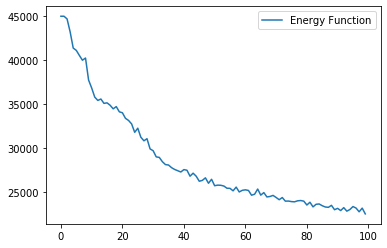
\includegraphics[scale=0.7]{hw3-2-graph1.png}
\begin{center}
\end{center}
\caption{Energy function\label{fig}}
\end{figure}
As expected the Energy function decreases over the span of the learning.  It is notable, that the learning in the beginning is much faster and later slows down. You can see the vanishing gradient problem in this slowing down, in the energy function, but also in the lack of change of the learning rate of each layer.

The learning rate of the different layers in the beginning has quite a variety. The closer the layer is to the output layer, the higher the learning rate is. But as the learning continues the learning rates converge and show a very similar course approximately from epoch 20  on.
The converging happens approximately for the first 20 episodes, where the layers with lower starting rate of learning show a much steeper increase until they finally reach the same level of learning rate as the other layers. 
\begin{figure}
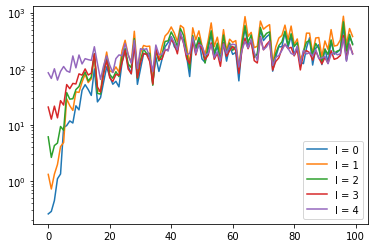
\includegraphics[scale=0.7]{hw3-2-graph2.png}
\begin{center}
\end{center}
\caption{Learning rate of each layer\label{tab}}
\end{figure}
\end{document}
